\documentclass[a4paper,12pt,abstracton,titlepage]{scrartcl}

\usepackage[french]{babel}
%\usepackage[T1]{fontenc}
\usepackage[utf8]{inputenc} % Umlaute, evtl. vom Betriebssystem abhaengig
\usepackage{lmodern}
\usepackage{pgfgantt}
\usepackage{titlesec}
\usepackage{float}
\usepackage{floatflt}
\usepackage{blindtext}
\usepackage{amsmath}
\usepackage{tabularx,url}
\usepackage[a4paper, left=2cm, textwidth=17cm, top=1.5cm]{geometry}
\usepackage{hyperref}
\usepackage{longtable}


\titleformat*{\section}{\large\bfseries}
\titleformat*{\subsection}{\large\bfseries}
\titleformat*{\subsubsection}{\large\bfseries}
\titleformat*{\paragraph}{\large\bfseries}
\titleformat*{\subparagraph}{\large\bfseries}

\renewcaptionname{french}{\figurename}{Fig.}

%\titlehead{Ulm University}
%\title{Title}
%\subject{Subject}
%\author{Author}
%\publishers{%
	%\rule{\textwidth}{0.4pt} \\
	%\vspace{0.5cm}
    %\normalfont\normalsize%
    %\parbox{0.9\linewidth}{%
    %    Abstract or Introduction
    %} \\
    %\vspace{0.5cm}
   	%\rule{\textwidth}{0.4pt}
%}
\title{Partajeux}
\date{26 janvier 2018}
%\author{DANG Hung Hoang,\\FUDITPHU Yan-Guillaume,\\KULZER Ulrike}
\author{John Doe\\ Magic Department, Richard Miles University
        \and Richard Row, \LaTeX\ Academy}

\renewcommand*\contentsname{Summary}

\begin{document}
%\maketitle

\begin{titlepage}
	\centering
	{\LARGE ESIEE Paris\par}
	\vspace{1cm}
	{\scshape\Large SI-4301B Architecture et développement d’applications Web en PHP\par}
	\vfill
	{\huge\bfseries Partajeux\par}
	\vfill
	{\large DANG Hung Hoang, FUDITPHU Yan-Guillaume, KULZER Ulrike\par}

\end{titlepage}



%%% begin costom title
{\Large\noindent \emph{ESIEE Paris}}

{\Large\noindent \emph{SI-4301B}}
\vspace{1cm}
\begin{center}
	{\huge \textbf{Partajeux}
	\\
	\vspace{0.3cm}
	\large DANG Hung Hoang, FUDITPHU Yan-Guillaume, KULZER Ulrike
	\\
	\vspace{0.2cm}
	\today}
\end{center}
%%% end custom title
\vspace{1cm}
%\maketitle
\tableofcontents

\setcounter{page}{1} % reset page counter to one for the first page, leave the title page out

\newpage
\section{Présentation du projet}
\subsection{Introduction/Description}
\vspace{0.2cm}
{\Large Partajeux\\}

Est une plateforme de mise en relation qui permet aux utilisateurs d'échanger
pour une durée de temps leur jeux vidéo en ligne. Ils déterminent grâce à
l'application les jeux qu'ils veulent échanger, puis fixent un rendez vous (date, heure, lieu de l'échange, durée).//
L'utilisateur doit pouvoir se connecter à l'application, s'identifier, ajouter ses jeux à échanger et ajouter des jeux voulu. L'utilisateur pourra rechercher les jeux qu'il veut et l'application affichera les utilisateurs qui peuvent potentiellement échanger (ils sont soit intéressés par un de nos jeux, soit ils ont la console pour un de nos jeux). L'utilisateur pourra ensuite proposer un échange et attendra la confirmation. Lorsque l'échange s'effectue les utilisateurs confirment l'échange et les jeux deviennent indisponible. Lorsque la durée de l'échange est terminé les utilisateurs doivent confirmer le retour des jeux pour qu'ils redeviennent disponible dans l'application.\\

Sites d'inspiration:\\
\begin{itemize}
\item Steam : 
\url{http://store.steampowered.com/}\\
\item Romstation : 
\url{http://www.romstation.fr/accueil}\\
\item Smiile : 
\url{https://www.smiile.com/}\\
\item MyTroc : 
\url{https://mytroc.fr/}\\
\item GchangeTout : 
\url{http://www.gchangetout.com/}\\
\item Ebay : 
\url{https://www.ebay.fr/}\\
\item LeBonCoin : 
\url{https://www.leboncoin.fr/}\\
\end{itemize}

\subsection{L'équipe}
% experiences
L'équipe de Partajeux se compose de trois membres :\\
\begin{itemize}
\item Hung Hoang DANG : expérimenté en développement web et SQL\\
\item Yan-Guillaume FUDITPHU : expérimenté en développement web et SQL\\
\item Ulrike KULZER : expérimentée en SQL\\
\end{itemize}



\newpage
\section{Analyse fonctionnelle}
\begin{longtable}{|p{0.23\textwidth}|p{0.25\textwidth}|p{0.25\textwidth}|l|}
\hline
\textbf{Fonctionnalité} & \textbf{Tâche} & \textbf{Sous-tâche} & \textbf{Importance}\\
\hline
Page de connexion & Formulaire d'inscription & Nom d'utilisateur & *****\\
 \hline
 & & Adresse Mail & *****\\
 \hline
 & & Mot de passe & *****\\
 \hline
 & & Taper deux fois & **\\
 \hline
 & & & \\
 \hline
 & Formulaire de connexion & Nom d'utilisateur & *****\\
 \hline
 & & Mot de passe & *****\\
 \hline
 & & Adress mail idenfiant & * \\
 \hline
  & & & \\
 \hline	
 & Description de l'application & Texte & ****\\
 \hline
 & & Image & **\\
 \hline
  & & & \\
 \hline
  & Information (Mention légale) &  Texte & ***\\
 \hline
 & & & \\
 \hline
 & & & \\
 \hline
Page d'accueil & Vous êtes connecté en tant que & & *****\\
 \hline
& Mes jeux & & *****\\
 \hline
& Jeux voulu & & *****\\
 \hline
& Barre de recherche & & *****\\
 \hline
& Notification & & ***\\
 \hline
  & & & \\
 \hline
 & & & \\
 \hline
Page de profil & Changer mot de passe & & *****\\
 \hline
 & Changer adresse mail & & *****\\
 \hline
 & Changer/ajouter photo de profil & & *\\
 \hline
 & bloquer utilisateur & & *\\
 \hline
 & & & \\
 \hline
 & & & \\
 \hline
Page de recherche & afficher résultat & afficher le jeu (titre, console, année,...) & *****\\
\hline
 &  & afficher les users dont l'échange est possible & *****\\
 \hline
 & afficher les propositions de résultats en temps réel &  & **\\
 \hline
 & & & \\
 \hline
 & & & \\
 \hline
Page description jeu & Image &  & ****\\
 \hline
 & Titre &  & *****\\
 \hline
 & Console &  & *****\\
 \hline
 & Année &  & ***\\
 \hline
 & Description &  & ******\\
 \hline
 & Proposition d'échange &  & ******\\
 \hline
 & & & \\
 \hline
 & & & \\
 \hline
Formulaire d'échange & Lieu &  & *****\\
\hline
 & Date et heure &  & *****\\
 \hline
 & Durée de l'échange &  & *****\\
 \hline
 & Jeux échangés &  & *****\\
 \hline
 & Noms des utilisateurs &  & *****\\
 \hline
 & Bouton confirmation et envoi à l'autre utilisateur &  & *****\\
 \hline
 & Pouvoir modifier la proposition (exemple : heure) et la renvoyer &  & ****\\
 \hline
 & Champ de texte &  & *****\\
  \hline
\end{longtable}


\section{Modèle conceptuel de données}
\vspace{0.5cm}
% E-R-Diagramme
\begin{minipage}[c]{\textwidth}
\centering
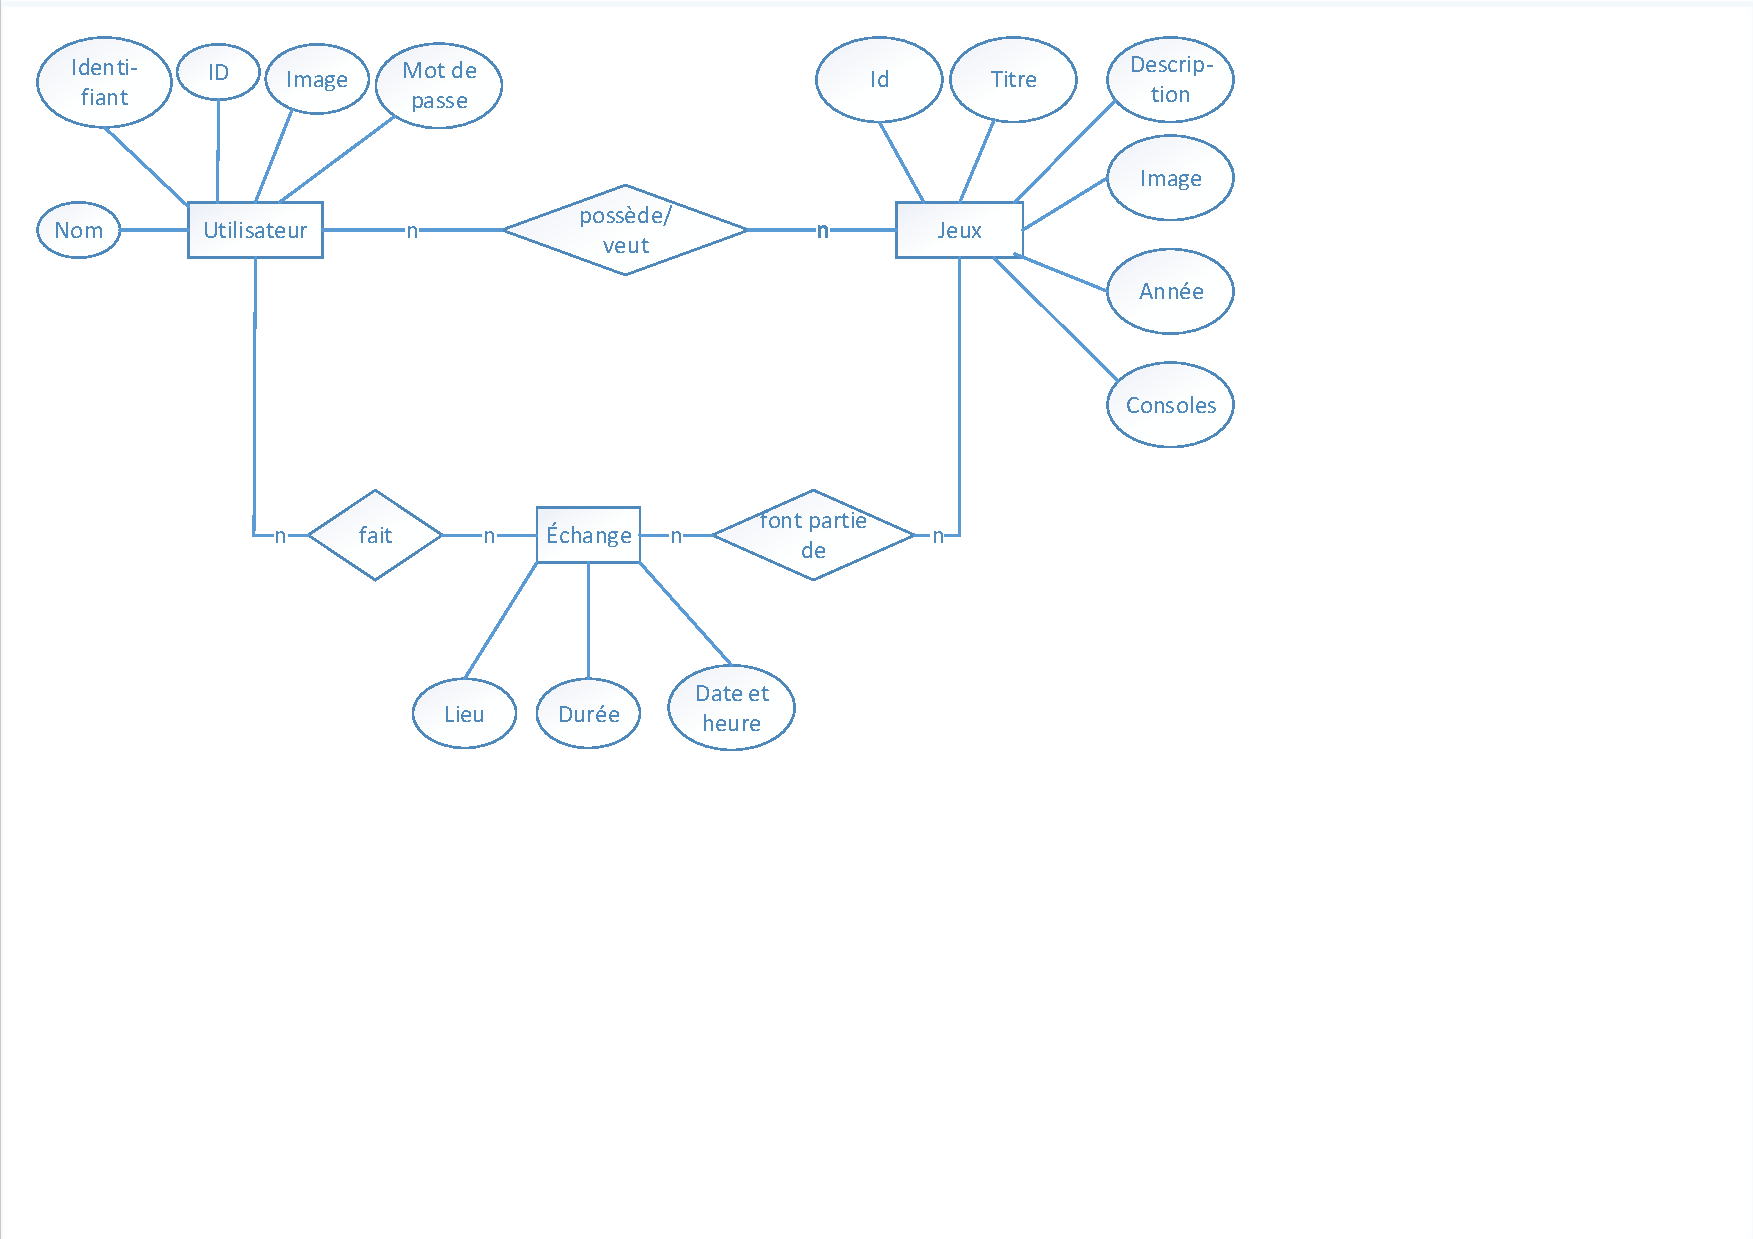
\includegraphics[width=\textwidth, trim=5mm 80mm 80mm 5mm, clip]{./doc/E-R-Diagrammme.pdf}
    %TRIM = LINKS UNTEN RECHTS OBEN
\captionof{figure}{Modèle entité-association au début du projet}
\label{img:er}
\vspace{1cm}

% Modèle conceptuel de données FINALE
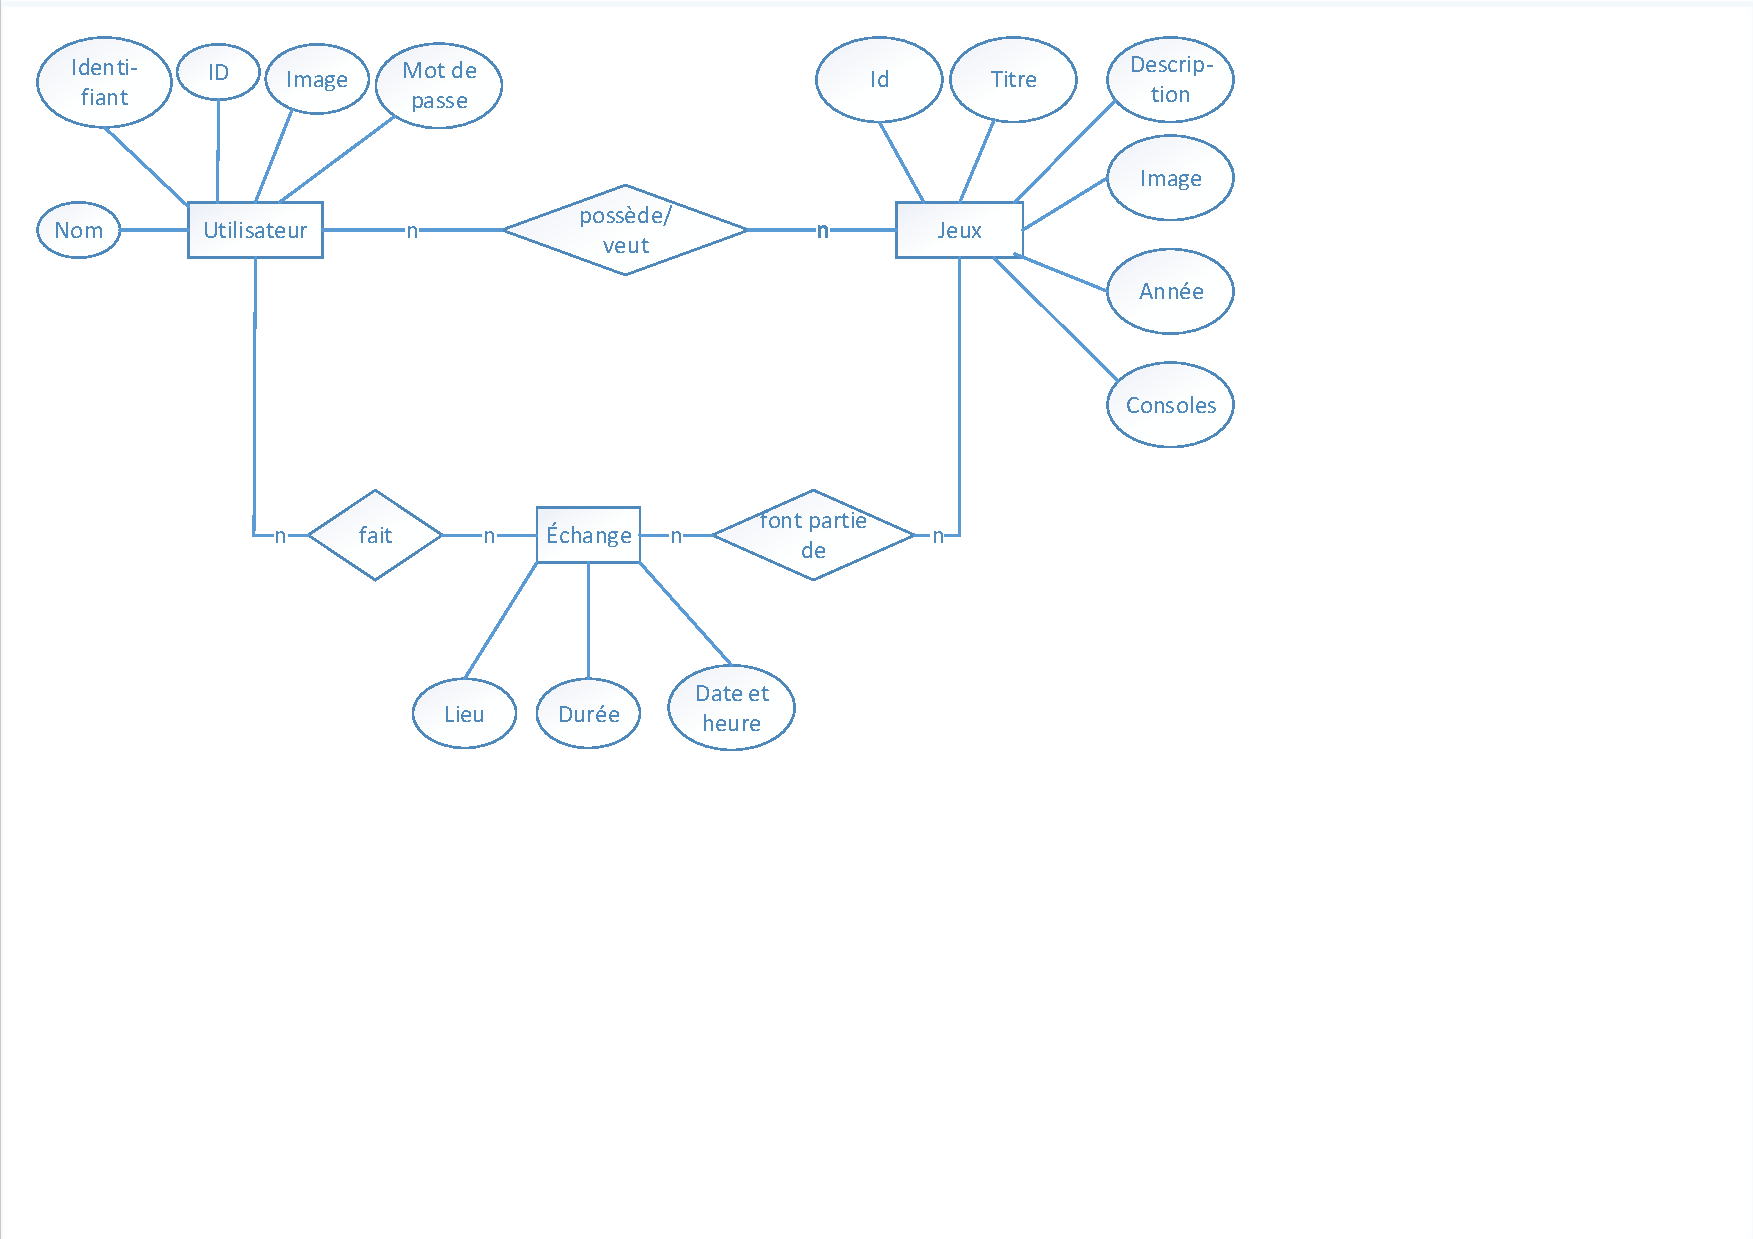
\includegraphics[width=\textwidth, trim=5mm 80mm 80mm 5mm, clip]{./doc/E-R-Diagrammme.pdf}
    %TRIM = LINKS UNTEN RECHTS OBEN
\captionof{figure}{Modèle conceptuel de données à la fin du projet}
\label{img:mcd}
\end{minipage}

\newpage
\section{Documentation}
\subsection{Documentation technique}
\subsubsection{Organisation}
Pour mieux nous organiser et échanger le code du programme nous avons décidé d'utiliser git. Git est un système de contrôle de versions distribuées gratuit qui était créé pour gérer vite et efficacement les projets de toutes les tailles. Pour notre projet nous avons utilisé un repository public.
Vous trouveriez plus des informations sous \url{https://github.com/} et \url{https://git-scm.com/}.
\subsubsection{Pré-requis et instruction d'installation}
-- apache, javascript, php, html, css, mySQL, jQuery

\subsubsection{Choix d'architecture et d'implémentation particuliers}
-- modèle MVC

\subsection{Documentation utilisateurs}
% captures d'écran
\textbf{Cette partie devra contenir un bref descriptif de l'application pour l'utilisateur final : description des menus et principales fonctionnalités. Vous pourrez y ajouter éventuellement des copies d'écran}\\
\paragraph{}
Lorsque l'utilisateur ouvre la page de Partajeux il se retrouve sur la page d'accueil suivante (voir \ref{}). Ici il peut trouver plus d'informations sur Partajeux en cliquant sur le bouton "Partajeux" dans la barre de navigation ou se connecter directement avec son identifiant et mot de passe. S'il n'est pas encore inscrit il suffit de cliquer sur "Inscription" ce qui va afficher le formulaire d'inscription (voir \ref{}). Pour s'inscrire l'utilisateur doit mettre son nom et son adresse mail. Ensuite il choisit un identifiant qui est utilisé pour se connecter et un mot de passe qu'il doit entrer deux fois pour éviter qu'il fait une faute et qu'il ne peut plus se connecter après. Le système va chercher dans la base de données si l'identifiant est déjà pris et dans ce cas prévenir l'utilisateur.
Une fois inscrit et connecté, l'utilisateur peut
\begin{itemize}
\item rechercher des jeux avec la barre de recherche qui propose des jeux correspondants à sa saisie
\item gérer ses jeux voulus
\item gérer ses jeux
\item gérer ses échanges
\end{itemize}






\begin{minipage}[t]{0.5\textwidth}

 %   \begin{center}
  %  \raggedleft
% 	\includegraphics[height=3.4cm]{}
 	%\caption{exemple du cryptage de Vigenère}
% 	\label{exVig}
%    \end{center} 
	
  \end{minipage} 
%  \begin{minipage}[t]{0.4\linewidth}
 %   \raggedleft
  %  \strut\vspace*{-\baselineskip}\newline\includegraphics[width=0.9\linewidth]{}
    %\caption{décalage de l'alphabet}
   % \label{cesar}
    %\paragraph{}
    %\strut\vspace*{-\baselineskip}\newline\includegraphics[width=0.9\linewidth]{}
    %\caption{tableau de Vigenère}
    %\label{tabVig}
  %\end{minipage}





%{\fbox{\parbox{\textwidth}{\raggedright
%\includegraphics{}}}
%	\captionof{figure}{Écran d'accueil}
%	\label{SP}
%}

%\begin{minipage}[c]{\textwidth}
%\centering
%    \includegraphics[width=\textwidth, trim=1mm 50mm 1mm 1mm, clip]{}
    %TRIM = LINKS UNTEN RECHTS OBEN
%    \captionof{figure}{Structure du programme en modules}
%    \label{img:structure}
%\end{minipage}


%\begin{floatingfigure}[l]{5.3cm}
%	\includegraphics[width=0.25\textwidth]{./Bilder/2venn.png}
%	\caption{Prinzip der additiven Farbmischung}
%	\label{venn}
%\end{floatingfigure}


%\par
%\vspace{0.5cm}

% "`Standard Definition Television"', HDTV für "`High Definition Television'".


%\begin{itemize}
%\item \blindtext
%\item \blindtext
%\end{itemize}
%\begin{enumerate}
%\item \blindtext
%\item \blindtext
%\end{enumerate}
%\begin{description}
%\item [Ant] \blindtext
%\item [Elephant] \blindtext

%\textbf{greatest} 
%\underline{science} 
%\textbf{\textit{accident}}.


\end{document}




% LABEL UNTER CAPTION

